\documentclass[../main.tex]{subfiles}
\begin{document}
\setchapterstyle{kao}
\setchapterpreamble[u]{\margintoc}
%Continue of L23 26/05/2022
\chapter[Representations of $\mathfrak{sl}(2,\mathbb{C})$ and $\mathfrak{su}(2)$]{Representations of $\mathfrak{sl}(2,\mathbb{C})$ and $\mathfrak{su}(2)$\footnotemark[0]}
\labch{RTsl2c}
\section{Motivation}
Why should we spend three hours of our life on this representation?
\subsection{Physical}
$\mathfrak{sl}(2,\mathbb{C})$ is the complexified version of $\mathfrak{su}(2)_{\color{red}{\mathbb{C}}}$
\[
\mathfrak{sl}(2,\mathbb{C})=\mathfrak{su}(2)_{\color{red}{\mathbb{C}}}
\]
In the sense that we consider elements of $\mathfrak{su}(2)_{\color{red}{\mathbb{C}}}$ and we allow \textbf{linear combinations with \underline{complex} coefficients}.\marginnote{This might seem strange, but this is something that we already did at the third year of the bachelor, when we did the theory of angular momentum. We considered $J_1$ and $J_2$ as the generators of the angular momentum
\[
J_1,J_2\in i\mathfrak{su}(2)
\]
and then at some point, we considered the combination
\[
J_{\pm}=J_1{\color{red}\pm i}J_2
\]
Maybe we did not notice at that time, but this is not an element of $\mathfrak{su}(2)$, because this latter is a real Lie algebra. Nevertheless, it is an interesting object, it is an element of the complification of $\mathfrak{su}(2)$. If we do a little bit of computation, we can discover that the complexification is exactly $\mathfrak{sl}(2,\mathbb{C})$} If we consider \textbf{complex} representations of $\mathfrak{su}(2)$ (as in QM) they are equivalent to representations of {\color{red}$\mathfrak{sl}(2,\mathbb{C})$}. We shifted the question to \textit{Why is $\mathfrak{su}(2)$ important?} But we already know the answer:
\[
\mathfrak{su}(2)
\begin{cases}
\textrm{Angular momentum } \ \mathfrak{su}(2)\cong \mathfrak{so}(3)\\
\textrm{Electroweak theory}
\end{cases}
\]
This is a motivation for physics, there is also the motivation that it is the universal covering of the Lorentz group.
\subsection{Mathematical}
There is a second motivation that comes from mathematics: when studying $\textrm{Irrep}(\mathfrak{g})$, $\mathfrak{g}$ semi-simple Lie algebra, this analysis relies on the fact that we find some relevant subalgebra of $\mathfrak{g}$ which are isomorphic to $\mathfrak{sl}(2,\mathbb{C})$. First we complexify our algebra, e.g. $\mathfrak{su}(2)$ and we find that it is exactly $\mathfrak{sl}(2,\mathbb{C})$. If we start with something strange, we complexify it, and then we could encounter inside it some subalgebras $\mathfrak{h}_k$ which are isomorphic to the special linear algebra, $\mathfrak{h}_j\simeq\mathfrak{sl}(2,\mathbb{C})$.
\section{Setting and notation}
First of all
\[
\dim_{\mathbb{C}}\mathfrak{sl}(2,\mathbb{C})=3
\]
Then we have to choose a basis. The canonical one is the following
\[
X=\mqty(\admat[0]{1,0}) \qquad Y=\mqty(\admat[0]{0,1}) \quad H=\mqty(\dmat[0]{1,-1})
\]
As exercise, compute the commutation relations, the results are
\begin{equation}\labeq{comm-gen-irr}
\comm{H}{X}=2X \qquad \comm{H}{Y}=-2Y \qquad \comm{X}{Y}=H
\end{equation}
We recognize something: we can suppose that $H$ is $J_3$, and $X\to J_+$, \\
$Y\to J_-$ up to $\frac{i}{2}$. This is the good occasion to emphasize that there is a schizophrenia in terminology between mathematics and physics, schematized in \reffig{schizzo-not}.
\begin{figure}[h!]
	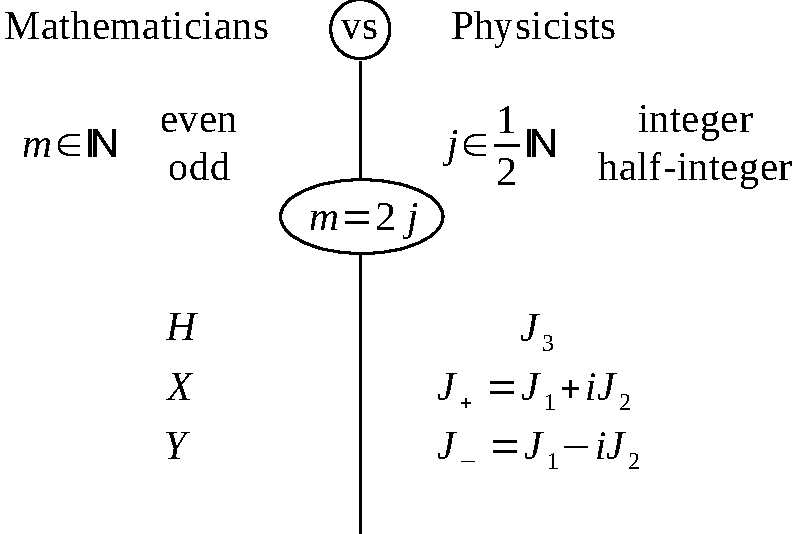
\includegraphics[width=1\linewidth]{images/schizzo_not.pdf}
	\caption[Schizophrenic terminology scheme between mathematics and physics]{$J_+$ and $J_-$ are not elements of $\mathfrak{su}(2)$, they are in the complexification. This is why are not claiming that they are equal, because there are some nasty factors.}
	\labfig{schizzo-not}
\end{figure}
\begin{exercise}
Compare with angular momentum theory (AMT) and translate the names of the objects.
\end{exercise}
\section{Main theorem}
\begin{theorem}\labthm{main-theo}
[Irreps of $\mathfrak{sl}(2,\mathbb{C})=\mathfrak{su}(2)_{\mathbb{C}}$] For every $m=2j\in\mathbb{N}$ there exists a \textbf{complex representation of} $\mathfrak{sl}(2,\mathbb{C})$ with dimension
$2j+1$. Any two \textbf{irreducible representations} with the same dimension are \textbf{equivalent/isomorphic}.
\end{theorem}
\paragraph{Main tool:} Ladder structure (struttura a scala).
\begin{figure}[h!]
	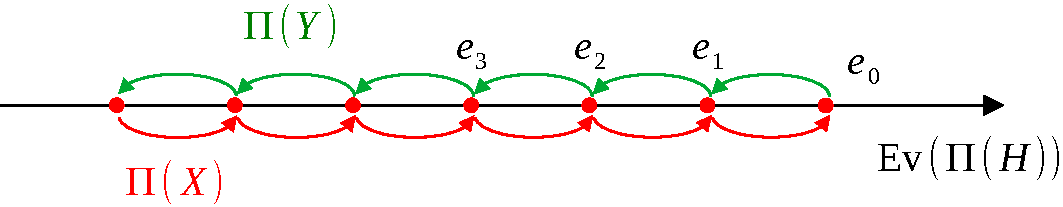
\includegraphics[width=1\linewidth]{images/ladder_Structure.pdf}
	\caption*{}
	\labfig{ladd-struc}
\end{figure}

We put on a line the eigenvalues of one of the operators: $\Pi(H)$. We have three generators, but they do not play all the same role. $H$ is used to label the eigenstate of the representation, while $X$ and $Y$ (or better their representative via $\Pi$) are used to increase or decrease the eigenvalue of the representation, as it happens with $J_+$ and $J_-$ in the analogous theory.  The eigenvalues will be finitely many numbers, because the dimension of $V$ is finite. Then we will notice that $\Pi(X)$ maps  every eigenvector in the eigenvector of the next eigenvalue. Similarly $\Pi(Y)$ will act in the opposite direction. 
\[
{\color{red}\longrightarrow \Pi(X)} \qquad {\color{Green}\longrightarrow \Pi(Y)}
\]
As the representation is finite dimensional, there should a be an endpoint in this ladder. We will characterize the end-point towards $+\infty$ and this will be our $e_0$; while going downstair we will construct $e_1,e_2,e_3$\marginnote{This labelling is not the same as the one of the angular momentum theory, but it is the one which is convenient for further generalization.}.

Let us emphasize that the ladder structure is quite universal. We already encountered different kind of ladders, e.g.:
\begin{enumerate}
    \item harmonic oscillator;
    \item Landau operator;
    \item angular momentum.
\end{enumerate}
\begin{lemma}[Ladder structure - Struttura a scala]\lablemma{Ladder-structure}\index{Ladder structure}Given the representation $\pi:\mathfrak{g}\to\textrm{End}(V)$, suppose $u\in V$ is eigenvector of $\pi(H)$ with eigenvalue $\alpha\in\mathbb{C}$. Then
\[
\star \quad \Big|\Big| \quad \pi(H)\left(\pi(X)u\right)=(\alpha\underset{\mathclap{\tikz \node {$\uparrow$} node [below=1ex] {\footnotesize plus};}}{+}2)\pi(X)u
\]
Then \textbf{\underline{either}} $\pi(X)u=0$ or
$\pi(X)u$ is eigenvector of $\pi(H)$ with eigenvalue $\alpha+2$.

Similarly:
\[
\pi(H)\left(\pi(Y)u\right)=(\alpha\underset{\mathclap{\tikz \node {$\uparrow$} node [below=1ex] {\footnotesize minus};}}{-}2)\pi(Y)u
\]
\end{lemma}
So, there are two possibilities, either the action of $\pi(X)$ increases the eigenvalues by $2$, or, if we are at some other point, it will die, i.e. it will become zero, as in \reffig{ladd-struc2}.
\begin{figure}[h!]
	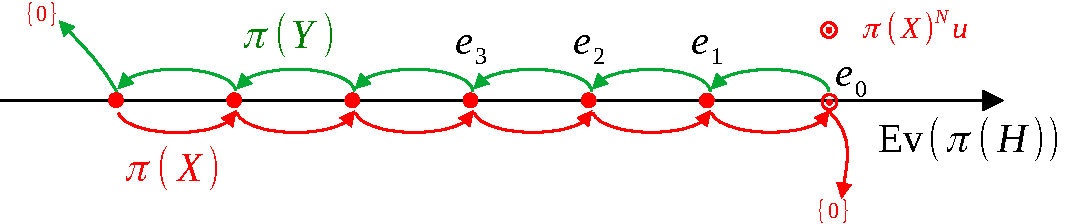
\includegraphics[width=1\linewidth]{images/ladder_Structure2.pdf}
	\caption{Ladder structure.}
	\labfig{ladd-struc2}
\end{figure}
The proof of the lemma is elementary.
\begin{proof}
We compute the commutator
\[
\comm{\pi(H)}{\pi(X)}\overset{\textrm{hom}}{=}\pi\left(\comm{H}{X}\right)\overset{(\ref{eq:comm-gen-irr})}{=}2\pi(X)
\]
Now we do the explicit computation
\WithArrowsOptions{displaystyle}
\[
\begin{WithArrows}
\pi(H)\pi(X)u
&=\pi(X)\overbrace{\pi(H)u}^{=\alpha u}+2\pi(X)u\Arrow{Everything is linear,\\so we collect the $\alpha$'s}\\
&=\left(\alpha+2\right)\pi(X)u
\end{WithArrows}
\]
This is all the algebra we need. We say either $\pi(X)$ is zero, or this is exactly the eigenvalue equation with eigenvalue $\alpha+2$. Similarly:
\[
\comm{\pi(H)}{\pi(Y)}={\color{red}\underset{\mathclap{\tikz \node {$\uparrow$} node [below=1ex] {\footnotesize minus};}}{-}}2\pi(Y)
\]
\end{proof}
We are ready to prove the main \refthm{main-theo}
\begin{proof}
Given a representation of the Lie algebra in the space of endomorphism of $V$, i.e. 
\[
\begin{split}
    \pi:&\mathfrak{g}\to\textrm{End}(V)\\
    &z\mapsto \pi(z)
\end{split}
\qquad \text{\parbox{3cm}{finite-dimensional\\{\color{red}Irreducible representation}}}
\]
We want to characterize its structure. Our strategy is to \textbf{diagonalize} {\color{red}$\pi(H)$}. We start saying that, as $V$ is a \textbf{\underline{complex}} vector space, $\exists$ eigenvector $u\in V$ with eigenvalue $\alpha\in\mathbb{C}$. Then we iterate the "Ladder \reflemma{Ladder-structure}":
\[
\pi(H)\pi(X)^ku={\color{red}\left(\alpha+2k\right)}\pi(X)^ku
\]
The point is that, since our space is finite dimensional {\color{red}$\dim V<+\infty$}, this sequence of vectors $\left\{\pi(X)^ku\right\}_{k\in\mathbb{N}}$ cannot be \textbf{all non-zero}.\marginnote{It can be proved that they are all linearly independent, otherwise we would have an infinite system of linearly independent vectors} Hence it must $\exists\;N$ such that
\[
\begin{split}
    {\color{red}u_0}=\pi(X)^Nu&\neq 0\\
    \pi(X)^{N+1}u&=0
\end{split}
\]
\marginnote{We must be on the extreme-right point in our map in \reffig{ladd-struc2}: $\pi(X)^Nu$. We decided to call it $u_0$.}The proof is by contradiction: suppose that such $N$ does not exist, then we have an infinite family of eigenvectors corresponding to different eigenvalues, which are linearly independent, then the space should be infinite dimensional, against the assumption.

Therefore, we set $\lambda:=\alpha+2N$, so that
\[
\begin{split}
    \pi(H)u_0&=\lambda u_0\\
    \pi(X)u_0&=0
\end{split}
\]
Now we go \textit{downstairs} along the ladder. It means that we apply and define
\[
{\star\quad \Big|\Big| \qquad \color{red}u_k:=\pi(Y)^ku_0\qquad \left(k\in\mathbb{N}\right)} 
\]
By applying again the Ladder \reflemma{Ladder-structure}, if we take
\[
\pi(H)u_k=\left(\lambda-2k\right)u_k
\]
As {\color{red}$\dim V<+\infty$}, then $\exists\;m:$
\[
\begin{split}
u_k&=\pi(Y)^ku_0\neq 0 \quad \forall k\leq m\\
u_{m+1}&=\pi(Y)^{m+1}u_0{\color{red}\;=0}
\end{split}
\]
But, as $u_{m+1}=0$, also $\pi(X)u_{m+1}=0$, which means:\marginnote{Here we used the fact (check by induction) that
\[
{\color{red}\pi(X)u_k=k\left[\lambda-\left(k-1\right)\right]u_{k-1}}
\]}
\[
0=\pi(X)u_{m+1}=\big[\underbrace{(m+1)}_{\neq 0}\underbrace{(\lambda-m)}_{=0}\big]\underbrace{u_m}_{\neq 0}
\]
Hence, we conclude that the eigenvalue is actually an integer ${\color{red}\lambda=m=2j\in\mathbb{N}}$.

\underline{Conclusion:} For every $\textrm{Irrep} \pi:\mathfrak{sl}(2,\mathbb{C})\to\textrm{End}(V)$ there exists ${\color{red}m=2j\in\mathbb{N}}$ and non-zero vectors $u_0,u_1,\dots,u_m$ in $V$ such that
\begin{equation}\labeq{struc-of-rep}
\textrm{\parbox{3cm}{Structure of $\pi$}}\quad\left|\quad
\begin{split}
\pi(H)u_k&={\color{red}\;\left(m-2k\right)\;}u_k\\
\pi(Y)u_k&=
\begin{cases}
u_{k+1}\quad &k<m\\
0\quad &k=m
\end{cases}\\
\pi(X)u_k&=
\begin{cases}
k\left[m-(k-1)\right]u_{k-1}\quad &k>0\\
0\quad &k=0
\end{cases}
\end{split}\right.
\end{equation}
As the $\textrm{Span}\{u_0,u_1,\dots,u_m\}$ is \textbf{invariant under} the action of the operators {\color{red}$\pi(H),\pi(X),\pi(Y)$} it is \textbf{invariant under} {\color{red}$\pi(Z)$} \textbf{for every} {\color{red}$Z\in\mathfrak{sl}(2,\mathbb{C})$}. Hence by irreducibility
\[
V=\textrm{Span}_{\mathbb{C}}\{e_0,\dots,e_m\}
\]
Therefore, the ${\color{red}\dim V=2j+1}$ and the structure of the representation is given by the formulas in \refeq{struc-of-rep}. If there are two irreducible representations
\[
\begin{split}
    \pi:\mathfrak{sl}(2,\mathbb{C})&\to\textrm{End}(V)\\
    \rho:\mathfrak{sl}(2,\mathbb{C})&\to\textrm{End}(W)
\end{split}
\]
with $\dim V=\dim W$ (hence we can identify $V\cong W$), then we construct an equivalence as in \reffig{equiv-class}
\begin{marginfigure}[-12mm]
	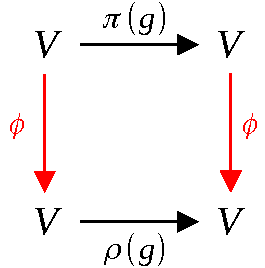
\includegraphics[width=1\linewidth]{images/equiv_class.pdf}
	\caption[Construction of the equivalence class $\phi$]{Construction of the equivalence class $\phi$. $w$ is identified with $g$.}
	\labfig{equiv-class}
\end{marginfigure}
By deciding that:
\[
\left\{
\begin{split}
\phi\pi(H)\phi^{-1}&=\rho(H)\\
\phi\pi(X)\phi^{-1}&=\rho(X)\\
\phi\pi(Y)\phi^{-1}&=\rho(Y)
\end{split}
\right.
\]
Since the structure is fixed and the three generators
are going to the three generators, then $\pi$ and $\rho$ are isomorphic.

We omitted the proof of the existence: \refthm{main-theo} <<\textit{... there \textbf{exists} a complex representation ...}>>. We did not do it, because actually we already encountered this representation in the theory of angular momentum. In the book of \sidecite{Hall2015_Ch4}, example 4.10, there is another kind of construction, which is more on the mathematical side.\marginnote[10mm]{The existence is important in mathematics, because from a set of assumptions which is the void set, we can deduce anything.}

\underline{Existence.} For every $m\in\mathbb{N}$, one exhibits a representation in ${\color{red}V_j=\mathbb{C}^{2j+1}}$ ${\color{red} \left(j\in\frac{1}{2}\mathbb{N}\right)}$.
\end{proof}

At home, compare what we saw here with the theory of angular momentum. Everything will be very similar, up to some annoying factors, as we mentioned. But there is an important difference, in this theory we truncated the ladder by the assumption that the representation is a finite-dimensional representation; while in QM we \textbf{do not} have this assumption. In QM, we take square-integrable functions over $\mathbb{R}^3$, we represent the group of rotations there and then we ask ourselves what happens. We have an operator $J^2$, which tells us which one is the good ladder to look at: the eigenstates of $J^2$ slice out Hilbert space in many little ladders, but then, how do we prove that the ladder terminates? We cannot know \textit{a priori} that the representation is finite-dimensional. Nevertheless, we have norms: our operators are operators in a Hilbert space. Hence, in particular we have the concept of \textbf{positive operator}, at some point we prove that some operators is a positive one ($J_+$ or $J_-$, do not remember), therefore it cannot have negative eigenvalues. So, the ladder should terminate, because otherwise this operator would have negative eigenvalues. This is the only difference between what we did here and the theory of angular momentum.
% FINE LEZIONE 23
%INIZIO LEZIONE 24 del 27/05 [DA ASCOLTARE LA REGISTRAZIONE]
\section{Lie groups VS Lie algebra representation}
\[
\begin{tikzcd}
\text{Lie group}\rar{\text{easy}} & \arrow[red, bend left]{l}[black,swap,below]{\color{red}\text{generally obstructed}} \text{Lie algebra}
\end{tikzcd}
\]
A Lie group representation $\Pi:\textrm{G}\xrightarrow[]{{\color{red}\text{Lie hom}}}\textrm{GL}(V)$ \textbf{induces a Lie algebra homomorphism} $\pi:\mathfrak{g}\xrightarrow[]{{\color{red}\text{Lie hom}}}\textrm{End}(V)$ such that \[
\Pi(e^x)=e^{\pi(x)}
\]
Explicitly, $\pi(x)=\dv{}{t}\Pi(e^{tx})\Bigr|_{\substack{t=0}}=\dd\Pi\Bigr|_{\mathbb{1}}(x)$.
%12:12
\begin{theorem}
If $G$ is a \underline{\textbf{simply connected}} (hence \textbf{connected}) Lie group with Lie algebra $\mathfrak{g}$, then \textbf{every} representation of $\mathfrak{g}$ induces a representation of $G$.
\end{theorem}
\begin{marginfigure}
    \centering
    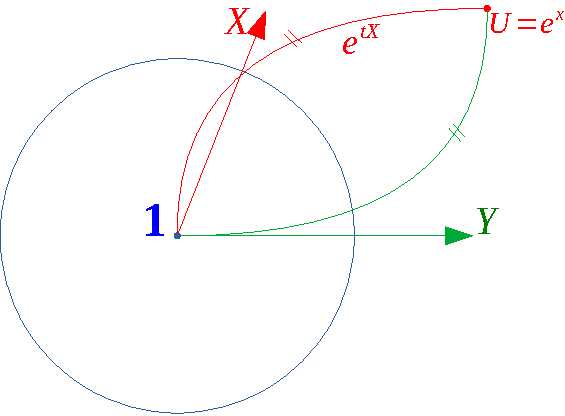
\includegraphics{images/Gsimplyconnected.pdf}
    \caption*{}
    \labfig{Gsimplyconnected}
\end{marginfigure}
\begin{example}
$G=\textrm{SU}(2)$:
\[
\text{irreps(SU(2))}\cong\text{irreps($\mathfrak{su}(2)$)}
\]
If $G$ is simply connected, the two points will lead to the \textbf{same extension} of $\Pi$ from U to $G$.
\end{example}
\underline{\textbf{Questions:}} what happens if $G$ is not simply connected? In general, $\textrm{irreps}(\mathfrak{g})\subsetneq\textrm{irreps}(G)$ (they are bigger and different).

What happens if $G=\textrm{SO}(3)$?
\begin{theorem}[$\textrm{irreps}(\textrm{SO}(3))$ is not $\textrm{irreps}(\mathfrak{so}(3))$]\index{$\textrm{irreps}(\textrm{SO}(3))$ is not $\textrm{irreps}(\mathfrak{so}(3))$}
Let $\sigma_m=\pi_m\circ\phi^{-1}$ as shown in \reffig{groupalgebra}. Then:
\begin{enumerate}
    \item if $m=2j$ \textbf{is even} ("\textbf{integer spin}"), then $\exists$ a representation \[\Sigma_m:\textrm{SO}(3)\xrightarrow[]{}\textrm{GL}(V_m\cong \mathbb{C}^{m+1})\] such that $\Sigma_m(e^x)=e^{\sigma_m(x)} \; \forall x\in\mathfrak{so}(3)$;
    \item if $m=2j$ \textbf{is odd} ("\textbf{half-integer spin}"), then such a representation $\Sigma_m$ does not exist.
\end{enumerate}
\end{theorem}
\begin{figure}[h!]
    \centering
    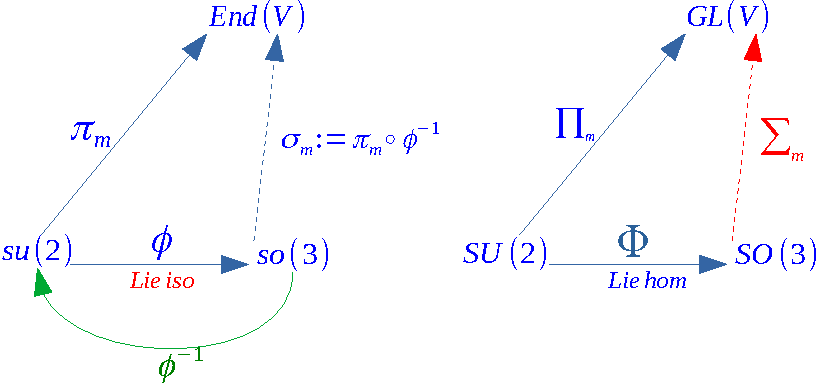
\includegraphics{images/groupalgebra.pdf}
    \caption[Lie algebra and Lie group]{\textbf{Left, Lie algebra}: $\phi$ is invertible! \raisebox{-\mydepth}{{
\includegraphics[height=1.1\baselineskip]{images/smile.jpg}}} irreps$(\mathfrak{su}(2))\cong$irreps$(\mathfrak{so}(3))$.\\
    \textbf{Right, Lie group}:$\Phi$ is \underline{not} invertible! \raisebox{-\mydepth}{{
\includegraphics[height=1.1\baselineskip]{images/anrgysmile.jpeg}}} $\ker\Phi=\{+\mathbb{1},-\mathbb{1}\}$.}
    \labfig{groupalgebra}
\end{figure}
\begin{proof}
of point 2. by contradiction.

Suppose $m=2j$ \textbf{is \underline{odd}} and that it $\exists$ a $\Sigma_m$ as above. Recall that a rotation along the axis $x_1$ is given by:
\[
e^{-i\theta F_1}=\left(\begin{array}{c:cc}
    1 & 0 & 0 \\
    \hdashline
    0 & \cos\theta & -\sin\theta\\
    0 & \sin\theta & \cos\theta
\end{array}\right) 
\qquad 
iF_1=\left(\begin{array}{c:cc}
    0 & 0 & 0 \\
    \hdashline
    0 & 0 & -i\\
    0 & +i & 0
\end{array}\right)
\qquad
e^{-2\pi iF_1}=\mathbb{1}
\]
On the other side, $\mathfrak{so}(3)\ni\sigma_m(F_1)=\pi_m(\phi^{-1}(F_1))$. After a little computation, we find that $\sigma_m(F_1)=\pi_m(E_1)$ where $E_1=\frac{i}{2}H$. Suppose $u_k$ is an eigenfunction of $\pi(H)$, hence it is an eigenfunction for $\frac{i}{2}\pi_m(H)=\sigma_m(F_1)$. Hence $\sigma_m(F_1)$ \textbf{is diagonalized on the basis} $\{u_0,u_1,\dots,u_k\}$:
\[
\sigma_m(F_1)=\left(\begin{array}{cccc}
    \frac{i}{2}m & & & \\
      & \frac{i}{2}(m-2) & & \\
      & & \ddots & \\
      & & & \frac{i}{2}(-m)
\end{array}\right)
\]
\underline{\textbf{Case I:}} $m$ \textbf{is odd} $\Rightarrow$ contradiction!
\begin{align*}
e^{2\pi\sigma_m(F_1)}&=\left(\begin{array}{ccc}
    -1 & & \\
     & \ddots & \\
     & & -1 
\end{array}\right)=-\mathbb{1}\\
\Sigma_m(e^{2\pi F_1})&=\qquad\Sigma_m(\mathbb{1})\qquad\quad=+\mathbb{1}
\end{align*}
\underline{\textbf{Case II:}} $m$ is even. For every rotation $R\in \textrm{SO}(3):\begin{cases}
\Phi^{-1}(R)=\{+U,-U\}\\
\Phi^{-1}(\mathbb{1})=\{+\mathbb{1},-\mathbb{1}\}
\end{cases}$, we define {\color{red}$\Sigma_m(R):=\Pi_m(U)$} and it is possible to check that it is a Lie group representation and that $\Sigma_m\circ\Phi=\Pi_m$.
\end{proof}
There is a nice story which an assistant of Wolfgang Pauli told to the professor about how this thing was born. Pauli was a famous physicist, but also an arrogant man. He wanted to build up a two-dimensional complex representation of the rotation group, because he knew, from spectroscopy data, that atomic states were two-fold (?) degenerates. He wanted to explain this fact in terms of representations of the group of rotations \textit{continue...} ahahah squid game. \raisebox{-\mydepth}{{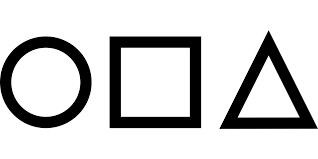
\includegraphics[height=1.1\baselineskip]{images/squidgame.png}}}
\end{document}